\documentclass[tikz,border=2pt]{standalone}
\usepackage{amsmath}
\usepackage{pgfplots}
\pgfplotsset{compat=1.18}
\usetikzlibrary{arrows.meta}
\begin{document}
% Constant force lambda = 0.02, delta = 0.03: the discounted death density v^t f_x(t) = 0.02 e^{-0.05t}.
% A 10-year term insurance keeps only the area on [0,10): 0.4(1 - e^{-0.5}) ~ 0.15739 of the whole-life total 0.4.
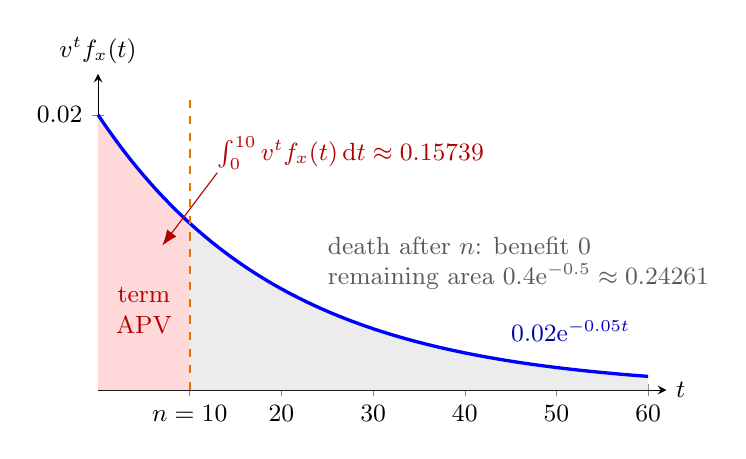
\begin{tikzpicture}[font=\small, >={Latex[length=2mm]}]
  \begin{axis}[
    axis lines=left, xmin=0, xmax=62, ymin=0, ymax=0.023,
    xtick={10,20,30,40,50,60}, xticklabels={$n=10$,$20$,$30$,$40$,$50$,$60$},
    ytick={0.02}, yticklabels={$0.02$}, scaled y ticks=false,
    xlabel={$t$}, ylabel={$v^tf_x(t)$},
    xlabel style={at={(axis description cs:1,0)}, anchor=west},
    ylabel style={rotate=-90, at={(axis description cs:0,1)}, anchor=south},
    samples=100, width=8.8cm, height=5.6cm, clip=false]
    \addplot[fill=red!15, draw=none, domain=0:10] {0.02*exp(-0.05*x)} \closedcycle;
    \addplot[fill=gray!15, draw=none, domain=10:60] {0.02*exp(-0.05*x)} \closedcycle;
    \addplot[blue, very thick, domain=0:60] {0.02*exp(-0.05*x)};
    \draw[orange!90!black, thick, dashed] (axis cs:10,0) -- (axis cs:10,0.0215);
    \node[red!70!black, align=center] at (axis cs:5,0.0058) {term\\APV};
    \node[red!70!black, anchor=west] at (axis cs:12,0.0172) {$\int_0^{10}v^tf_x(t)\,\mathrm{d}t\approx0.15739$};
    \draw[red!70!black, ->] (axis cs:13,0.0158) -- (axis cs:7,0.0105);
    \node[gray!70!black, anchor=west, align=left] at (axis cs:24,0.0092) {death after $n$: benefit $0$\\remaining area $0.4\mathrm{e}^{-0.5}\approx0.24261$};
    \node[blue!70!black, anchor=south west] at (axis cs:44,0.0028) {$0.02\mathrm{e}^{-0.05t}$};
  \end{axis}
\end{tikzpicture}
\end{document}
